\documentclass[11pt]{article}
\usepackage[margin=1in]{geometry}
\usepackage[T1]{fontenc}
\usepackage{lmodern}
\usepackage{microtype}
\usepackage{graphicx}
\usepackage{flafter}
\usepackage{placeins}
\usepackage{booktabs}
\usepackage{array}
\usepackage{amsmath,amssymb}
\usepackage{natbib}
\usepackage[hidelinks]{hyperref}
\usepackage{enumitem}
\setlist{nosep}
\newcolumntype{L}[1]{>{\raggedright\arraybackslash}p{#1}}

\title{From Scalar Reward to Cellular Credit: Separating Representation Selection from Neuron-Specific Learning}
\author{Ognjen \v{C}adovski\\
\small Doctoral student, Faculty of Mathematics, University of Belgrade\\
\small Supervisor: Aleksandar Taka\v{c}i\\
\small \texttt{ognjencadovski@gmail.com}}
\date{September 2026}

\begin{document}
\maketitle

\begin{abstract}
Learning from a scalar outcome leaves two distinct problems. A learner must identify which population representation produced the outcome, and it must determine how individual cells should change. Recent brain--computer interface evidence identified role-dependent dendritic signals consistent with neuron-specific instruction \citep{francioni2026}. We asked whether an ART-style top-down process could account for those signals without receiving an explicit neuron-wise error. A sequence of closed-loop simulations first tested pART-inspired representation selection, learned expectations, and local SMART-inspired plasticity. These mechanisms learned useful behavior, but their neuron-by-neuron topology came mainly from patterns already present in a fixed repertoire, and the complete model failed its preregistered longitudinal test. A generic node-perturbation comparator then showed that scalar reward can support arbitrary cellular learning when each cell retains a private eligibility trace. Finally, a common Francioni-inspired benchmark compared fixed-repertoire ART, local eligibility, their direct hybrid, a random control, and a privileged vector oracle on 32 held-out mappings. ART, eligibility, and the hybrid all improved behavior. ART selected useful pre-existing patterns. Eligibility created a new cellular topology. The hybrid combined these abilities, but its dendritic-like signal had the wrong sign and failed the frozen Francioni-like criteria. Only the privileged vector oracle passed the complete benchmark. The results therefore support a computational dissociation rather than an equivalence. Population selection and cellular credit may be complementary operations, but combining them does not by itself explain the measured biological signal.
\end{abstract}

\section{Introduction}
Many theories of learning begin with an error. They compare a desired outcome with the outcome that occurred, then use the difference to determine how the network should change. This approach is powerful because it connects behavior to adjustments at individual units or synapses. Its biological implementation is uncertain. The brain must obtain appropriately structured teaching information and deliver it to the cells that can improve the outcome.

A different tradition begins with population representations. Adaptive Resonance Theory (ART) describes how neural systems learn stable categories, form top-down expectations, and search when an expectation does not match current input \citep{carpenter1987}. Predictive ART (pART) extends this view to structural and temporal credit. It asks which maintained representation predicted a later consequence and should therefore be reinforced \citep{grossberg2018}. Learning is not described primarily as the minimization of a neuron-wise error.

The original motivation for this study came from encountering the findings of Francioni et al. during research on ART-style learning. Their closed-loop brain--computer interface (BCI) task revealed dendritic signals whose signs depended on the causal roles of individual neurons \citep{francioni2026}. The signals contained reward- and error-related information, predicted later changes in neural activity, and were necessary for learning under the reported perturbation. These observations are naturally discussed as neuron-specific error or target signals. Yet they also involve top-down input to dendritic compartments. This suggested a direct question. Could an apparently error-driven cellular result be the expression of a population-level learning process of the kind described by ART?

We made that question computationally specific. Could a pART-selected causal representation learn and express a top-down pattern that reproduced the neuron-specific, longitudinal signature reported by Francioni et al., even though the learner received no explicit neuron-wise error? pART was a reasonable starting point because it addresses delayed structural credit. ART supplies learned expectations. SMART supplies a model of apical feedback, matching, timing, and local plasticity \citep{grossbergversace2008}. Combining these components suggested a possible route from a delayed scalar outcome to cell-specific change. It did not guarantee that the route contained enough information.

That possible information gap is the central problem examined here. An outcome can arrive after the action that caused it, creating a temporal credit problem. Many cells can also be active at once while contributing differently to the outcome, creating a structural credit problem. A single scalar reward reports whether the joint action helped. On its own, it does not identify the contribution of each cell.

We call selection at the population level \emph{representation credit}. It means choosing and reinforcing a useful activity pattern that is already available to the system. We use \emph{cellular credit} for the finer problem of deciding the sign and size of change at each cell. The arrangement of those cell-specific effects is called the \emph{topology} of the learned signal. A system can solve representation credit without constructing a new cellular topology.

This distinction is especially important in a BCI task in which nearby cortical cells have opposite causal roles. One possible learning mechanism computes or supplies a different teaching value for every neuron. Another broadcasts one scalar outcome and combines it with information stored locally at each cell. A third selects a useful population pattern that already exists. These mechanisms can produce similar behavior, but they solve different problems.

We addressed that question through a sequence of computational studies. Each study addressed a limitation of the preceding one. We first asked whether selective feedback could route an opponent pattern that was already built into the model. We then hid cellular identity and required the model to select from random population patterns. Next, the model learned its own top-down expectation instead of receiving a copied pattern. A reduced local plasticity mechanism was tested on its own before it was added to the complete model. We then traced the source of the neuron-by-neuron pattern learned by that model. A generic study tested whether a local record of recent exploration could supply the missing cell-specific information. The final benchmark placed ART selection, local eligibility, and their hybrid in the same Francioni-inspired task and required them to satisfy behavioral, topological, and dendritic criteria separately.

This order is important. Successful behavior alone does not reveal whether the learner selected an existing representation or discovered how individual cells should change.

The contribution is therefore not a new general learning algorithm. It is a controlled comparison of explanatory levels. The experiments separate representation selection from cellular sign learning, test prospective dendritic criteria, and ask whether a direct combination of the two operations closes the explanatory gap. All numerical results and figures come from the archived repository record. Claims about published theory and biology are supported separately by external citations.

\section{Related work}
\subsection{Error, target, and dendritic accounts}
Backpropagation solves credit assignment in artificial networks by using the derivative of an objective to calculate coordinated weight changes. Biologically motivated alternatives replace exact backpropagation with feedback signals that can be processed locally. Multi-compartment models use basal dendrites for feedforward activity and apical dendrites for teaching or target-related feedback \citep{guerguiev2017,payeur2021}. These models show how segregated dendritic compartments can coordinate learning across layers. They still require a feedback signal whose structure is informative for the receiving cells.

Francioni et al. provided an experimental point of contact for this theoretical work \citep{francioni2026}. Their BCI task assigned opposite causal roles to intermingled cortical neurons. Soma-conditioned dendritic signals reflected those roles and predicted later activity change. Perturbing the relevant dendritic processing impaired learning. The study establishes a neuron-specific dendritic signal consistent with vectorized instruction. It does not determine the algorithm that constructs the vector, and it leaves open whether the measured activity is a teaching signal for synaptic change or a moment-to-moment computational signal.

\subsection{Learning from scalar reward and local variation}
A scalar reward can support neuron-specific learning when it is combined with a second quantity that varies across neurons or synapses. REINFORCE formalized stochastic policy updates from a global performance signal \citep{williams1992}. Node perturbation estimates a useful direction by correlating local exploratory changes with changes in an objective \citep{fiete2006}. Eligibility traces preserve locally available information until a delayed modulatory signal arrives \citep{izhikevich2007,gerstner2018}.

This principle has already been applied to BCI learning. A reward-modulated Hebbian model combined global reward with neuronal noise and reproduced selective network reorganization observed during a brain-control task \citep{legenstein2010}. The local-eligibility comparator used later in the present study belongs to this established family. Its purpose is not to introduce node perturbation as a new algorithm. It tests whether the information missing from the pART-inspired model is sufficient to explain arbitrary cellular roles in the same abstract task.

\subsection{ART-style representation credit}
ART addresses the stability--plasticity problem through category matching, vigilance, reset/search, and learned top-down expectations \citep{carpenter1987}. pART emphasizes structural and temporal credit at the level of maintained causal representations. A representation can be selected, preserved across a delay, and reinforced by broad motivational signals \citep{grossberg2018}. These mechanisms motivate representation-level credit but do not, by themselves, specify an arbitrary neuron-resolved feedback vector.

SMART provides a more cellular circuit motif. In a visual thalamocortical setting, learned higher-to-lower feedback reaches apical dendrites, a match-dependent on-center/off-surround circuit changes timing and participation, and a local voltage/conductance-gated rule changes synapses \citep{grossbergversace2008}. Canonical laminar extensions describe related modulatory feedback motifs \citep{grossberg2021}. Grossberg's vector associative motor systems address a different information boundary. They use an available target-versus-present difference vector \citep{gaudiano1991}. Importing such a vector into the present task would assume the neuron-specific information that the simulations are intended to explain.

The literature therefore suggests three accounts that must be distinguished. A feedback system may compute or transmit cell-wise error or target information. A representation-level system may reinforce a useful distributed pattern already present in a repertoire. A local exploratory system may combine a common scalar advantage with a cell-specific eligibility trace. The experiments below ask whether the second account can reproduce the cellular signature usually associated with the first. When it cannot, the third account identifies one established source of the missing information.

\section{Materials and methods}
\subsection{Task and available information}
The experiments used abstract closed-loop BCI tasks based on the information structure of the Francioni paradigm rather than a detailed reconstruction of its cortical circuit. Each cell had a hidden causal role $c_i\in\{-1,+1\}$, and the two roles occurred equally often. For a somatic population pattern $y$, the environment calculated a signed population drive equivalent to the difference between the mean activity of the P+ and P- groups. In the later standardized tasks this was
\begin{equation}
 u=\frac{2}{N}\sum_{i=1}^{N}(y_i-0.5)c_i.
\end{equation}
The drive changed a bounded visual state over several closed-loop action frames. The learner then passed through irrelevant distractor steps before receiving a scalar measure of improvement and a binary success signal. Some studies used two observable contexts. In the second context the same cells had the opposite causal roles.

The learner could observe the context, visual state, its own activity, permitted local variables, and the delayed scalar outcome. It could not observe the hidden role vector $c$. That information was used only in labeled positive controls and offline analyses. We measured task performance, alignment between learned patterns and hidden roles, recovery after the roles were changed independently, and the effects of removing proposed causal mechanisms. An alignment of 1 indicates a perfect match with the hidden roles. We use \emph{remapping} for an independently sampled change in those roles.

The theory-led models contain five quantities. The selected representation is $H_{k,h}$. Its learned top-down expectation is $T_{k,h,i}$. The modeled dendritic input is $D_i$, the plastic lower weight is $W_i$, and the somatic output is $S_i$. The main preregistered test asked whether an early dendritic signal predicted a later weight change and whether that weight change predicted a later change in somatic output. The predicted sequence was
\begin{equation}
 D^{\mathrm{early}}_{\mathrm{residual},i}\;\longrightarrow\;\Delta W_i\;\longrightarrow\;\Delta S_i.
\end{equation}
The test was evaluated while holding the selected hypothesis fixed. This prevents a switch between population patterns from appearing to be a change within individual cells. The dendritic measure was a \emph{residual}, meaning the part of the modeled dendritic signal left after accounting for somatic activity.

The SMART-derived models used the following qualitative plasticity rule.
\begin{equation}
 \Delta W_{jk}\propto f_G(V_k,\bar g_{jk})\left[\bar g_{jk}f_N(V_k)(\widehat w-\check w)+w_0-w_{jk}\right].
\end{equation}
In words, a synaptic weight changes according to conductance, voltage, spike timing, and the weight's current value \citep{grossbergversace2008}. These are quantities available at or near the modeled synapse.

The generic local-eligibility comparator used a different update. It is a simplified three-factor rule based on node perturbation. It is not a new learning algorithm \citep{fiete2006,izhikevich2007,gerstner2018}.
\begin{equation}
 \Delta A_i=\eta_N(R-b)e_i.
\end{equation}
Here, $R-b$ is the same scalar reward advantage for every cell. The eligibility trace $e_i$ is a short-lived record of cell $i$'s own exploratory perturbation. Because this trace differs across cells, the same reward can produce different local updates. The factor $\eta_N$ corrects known population-mean scaling. Hidden roles do not enter the update.

\subsection{Common Francioni-inspired benchmark}
The final benchmark used the same information boundary for every ordinary model. Ten cells were divided into five hidden P+ and five hidden P- roles. Their opponent activity moved a continuous visual state that was displayed in seven bins. A trial lasted at most 28 one-second action frames. The learner observed the displayed state and its change during the trial, followed by a delayed binary reward. It never observed the hidden role vector. Acquisition and an independently sampled hidden remap each lasted 14 blocks of 64 trials.

Five primary models were compared. The vector oracle received the hidden roles and served only as a sensitivity control. The ART learner selected from a fixed bank of 64 random balanced population patterns and learned top-down expectations. The eligibility learner used local perturbations and scalar visual and reward signals to adjust a cell-wise correction. The hybrid added that correction to the ART-selected pattern. The random model did not learn. Outcome shuffling, removal of exploration, removal of the temporal trace, and disabling eligibility in the hybrid provided causal controls.

Behavioral success was not treated as evidence of a dendritic teaching signal. Each model exposed its own genuine cell-indexed feedback quantity $F_i(t)$. The common observation layer generated a synthetic dendritic measurement
\begin{equation}
D_i(t)=\alpha S_i(t)+\beta\,\mathrm{standardize}\!\left(F_i(t)\right)+\epsilon_i(t).
\end{equation}
A separate linear soma--dendrite relation was then fitted for each cell, and the residual was analyzed. The frozen endpoints tested behavior, topology, role-by-direction vectorization, outcome decoding, prospective prediction of later activity, and preservation after matching somatic activity when matching was identifiable. ART and eligibility components in the hybrid were archived separately. This observation layer is a common measurement test, not a model of calcium biophysics.

\subsection{Experimental sequence and reproducibility}
The simulations were implemented in Python. Population-level experiments used NumPy \citep{harris2020}. The reduced spiking and local-plasticity motif used Brian2 \citep{stimberg2019}. Randomness was generated from explicit seeds, and paired conditions shared the same hidden roles and initial repertoires. Later studies used frozen held-out seed sets, preregistered effect floors, explicit positive controls supplied with hidden vector information, and causal ablations that shuffled outcomes, removed exploration, or removed eligibility. Table~\ref{tab:registry} provides the manuscript-level crosswalk to the repository's internal identifiers. The Results retain this chronology but use scientific study names in the narrative.

\begin{table}[tbp]
\centering\small
\begin{tabular}{L{0.11\linewidth}L{0.25\linewidth}L{0.14\linewidth}L{0.38\linewidth}}
\toprule
Registry ID & Study & Held-out units & Purpose \\
\midrule
EXP000 & Prestructured opponent-code routing & 30 seeds & Route an already available pattern. \\
EXP001 & Random-repertoire selection & 30 mappings & Test scalar selection and delayed representation credit. \\
EXP002 & Learned top-down expectancy & 30 mappings & Test whether an expectation supplies the longitudinal cellular signal. \\
EXP003 & Theory-to-code audit & Source audit & Identify supported links and unresolved mappings. \\
EXP003a & Reduced SMART motif & Mechanism tests & Isolate feedback, timing, and local plasticity. \\
EXP003b & Integrated composition & 12 mappings & Test the complete theory-led chain. \\
EXP004 & Origin of learned topology & 16 mappings & Separate construction from inheritance of repertoire geometry. \\
EXP005 & Local eligibility & 16 mappings per $N$ & Audit the published mechanisms, then test generic cellular credit. \\
EXP006 & Common Francioni-inspired benchmark & 32 mappings & Compare selection, cellular learning, and their direct hybrid under one frozen assay. \\
\bottomrule
\end{tabular}
\caption{Crosswalk between repository identifiers and the scientific studies described in the manuscript.}
\label{tab:registry}
\end{table}

\subsection{Statistical analysis}
The hidden mapping and its paired initial conditions formed the independent unit in confirmatory comparisons. Unless otherwise noted, intervals from the earlier studies are 95\% nonparametric bootstrap intervals obtained by resampling those units 5,000 times. EXP006 reports 95\% normal intervals across its 32 held-out mappings. Its pass or fail classification used scenario means and numerical floors committed before those mappings were accessed. Controls were designed to answer different failure modes. Hidden-vector controls established that the task and longitudinal assay were learnable when cell-wise information was supplied. Contextual bandits tested whether behavior required ART category dynamics. Outcome shuffling tested whether local traces remained correctly paired with consequences. Removing exploration or eligibility tested the two neuron-local components of the generic update. Exact replay analyses checked whether recorded legal variables reconstructed learned quantities.

\subsection{Scope of the claims}
Quantitative statements labeled as results are derived from committed protocols, frozen analyses, held-out records, or explicitly identified post-hoc audits in the project repository \citep{pvcRepo}. EXP006 was designed prospectively after the earlier synthesis exposed a gap between the motivating question and the existing experiments. Its protocol, parameters, source hashes, endpoints, and pass floors were frozen before confirmatory execution. The prestructured study tests routing, not de novo sign learning. Conclusions from theory-led studies apply to the implemented compositions and endpoints rather than to all ART, pART, or SMART models. The local-eligibility comparator is a generic three-factor rule and is not attributed to Grossberg. Biological interpretations remain hypotheses unless supported by the cited experimental literature.

\subsection{Link to published theory}
We compared every implemented step with the cited sources. pART motivated representation selection and maintenance. ART motivated expectation learning and match/reset. SMART motivated apical feedback and timing-dependent local plasticity. The dendritic measure was motivated by Francioni et al. The sources did not explain how a scalar outcome alone could create an arbitrary neuron-by-neuron mapping from $H$ to $T$. They also did not establish two biological mappings used by the model. The first links the SMART surround to NDNF-sensitive dendritic signals. The second links modeled current or voltage to a soma-conditioned calcium residual. These gaps motivated the later tests of topology and local eligibility.

\FloatBarrier
\section{Results}
\subsection{Routing a pattern already present}
The first study corresponds to registry record EXP000. It asked whether selective feedback could express opposite effects in two groups of cells when the required pattern was already built into the model. After two retained calibration attempts, the corrected model reached a late-task accuracy of 0.978 across 30 seeds. P+ modulation was $+0.673$, and P- modulation was $-0.673$ (Figure~\ref{fig:routing}). Their difference, the opposition index, was $+1.346$. Selective feedback could therefore route a strong opponent pattern without receiving a separate error value for every neuron on each trial.

This was an existence proof, not a test of cell-specific learning. P+/P- identity could be recovered from even and odd neuron indices, and that same identity was encoded in the category templates. Freezing category and value learning did not reduce accuracy. Every ordinary corrected trial matched a stored category, and none triggered a reset (Table~\ref{tab:supporting}). The model could use a pattern that it already possessed. It did not explain how that pattern could be found when cellular identity was hidden.

\begin{figure}[tbp]
\centering
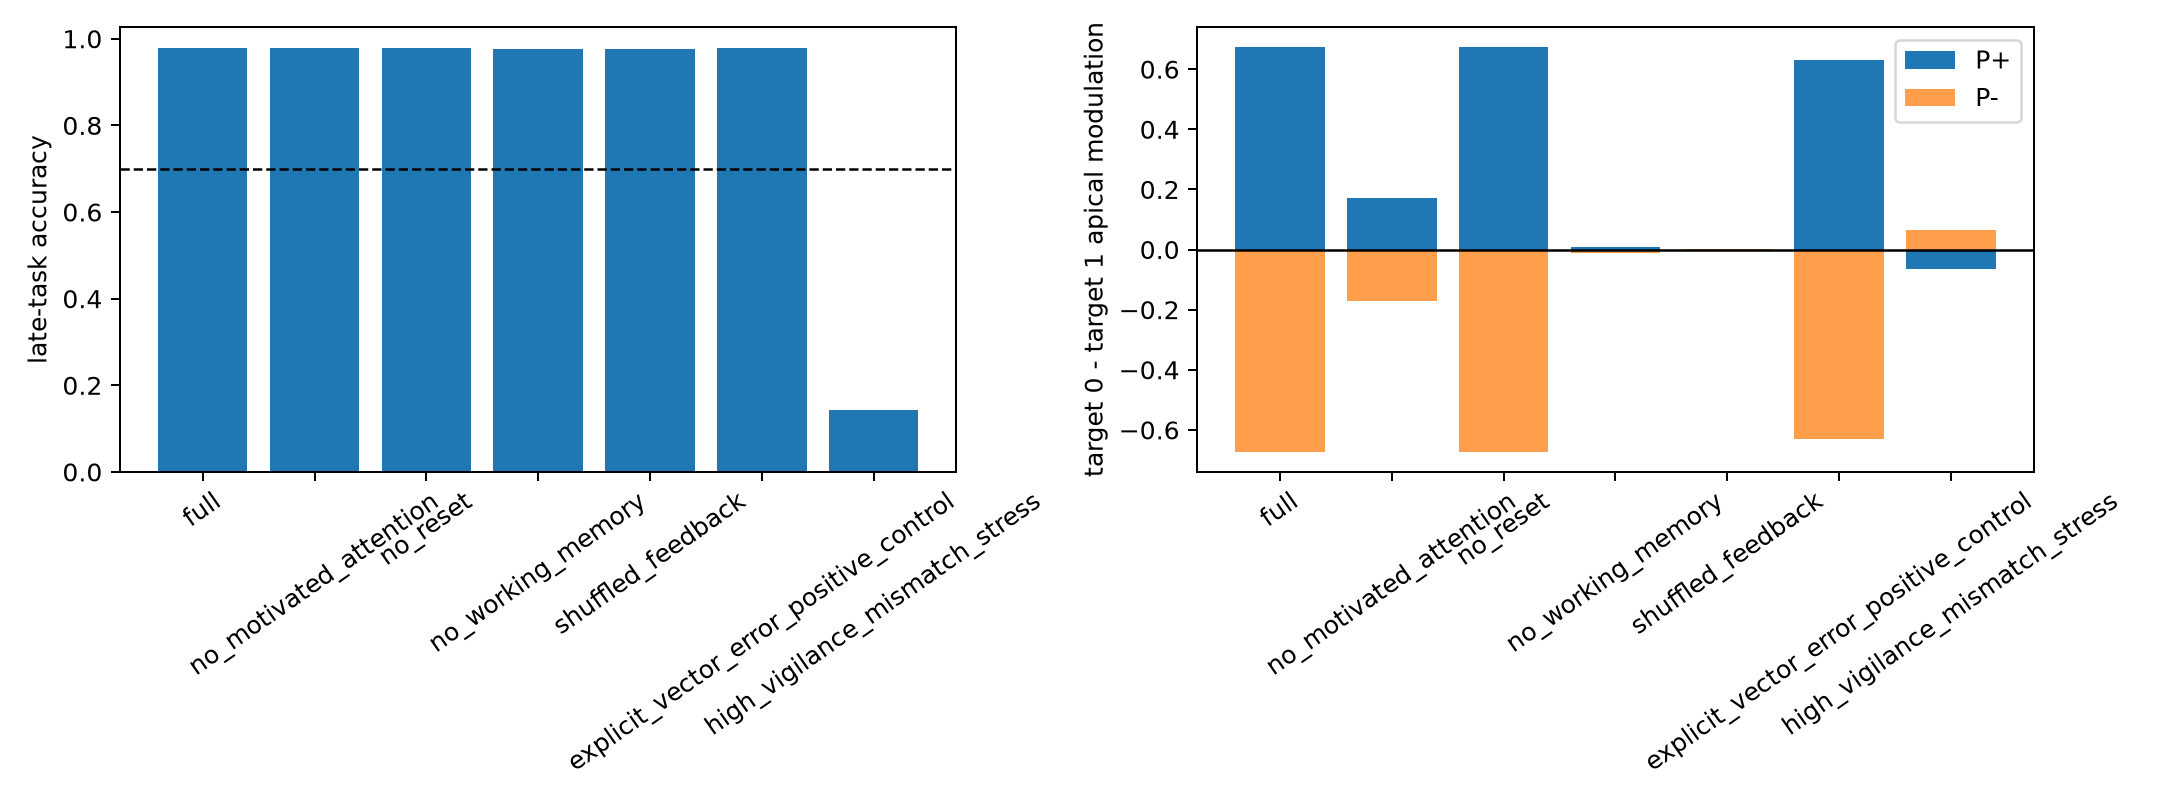
\includegraphics[width=\linewidth]{../results/initial_experiment.png}
\caption{Repository-derived summary of prestructured routing. Late-task accuracy remains high under several ablations because the opponent pattern is already present in the model. Shuffled feedback disrupts P+/P- modulation, while the explicit vector control serves as a positive control.}
\label{fig:routing}
\end{figure}

\subsection{Selecting from a random repertoire}
The next study (EXP001) hid population identity and replaced the opponent template with a bank of random patterns. It asked whether a scalar outcome could select a useful pattern, preserve it across irrelevant events, and support selection of another useful pattern after the hidden roles changed. The model succeeded at all three tasks.

Success depended strongly on what the random bank contained. Larger banks were more likely to include a pattern that already aligned well with the hidden roles, and the best initial alignment increased with bank capacity (Figure~\ref{fig:repertoire}). This result places the achievement at the representation level. Reinforcement selected a useful direction, but that direction had to be present before learning began.

The dendritic residual did not resolve the remaining cellular-credit problem. Its instantaneous alignment with hidden roles also appeared in controls that did not learn, and it did not reliably predict later cell-specific activity change. A positive control supplied with a separate teaching value for every neuron did predict that change. The next study asked whether a learned top-down expectation could generate the missing signal without receiving the hidden role vector.

\begin{figure}[tbp]
\centering
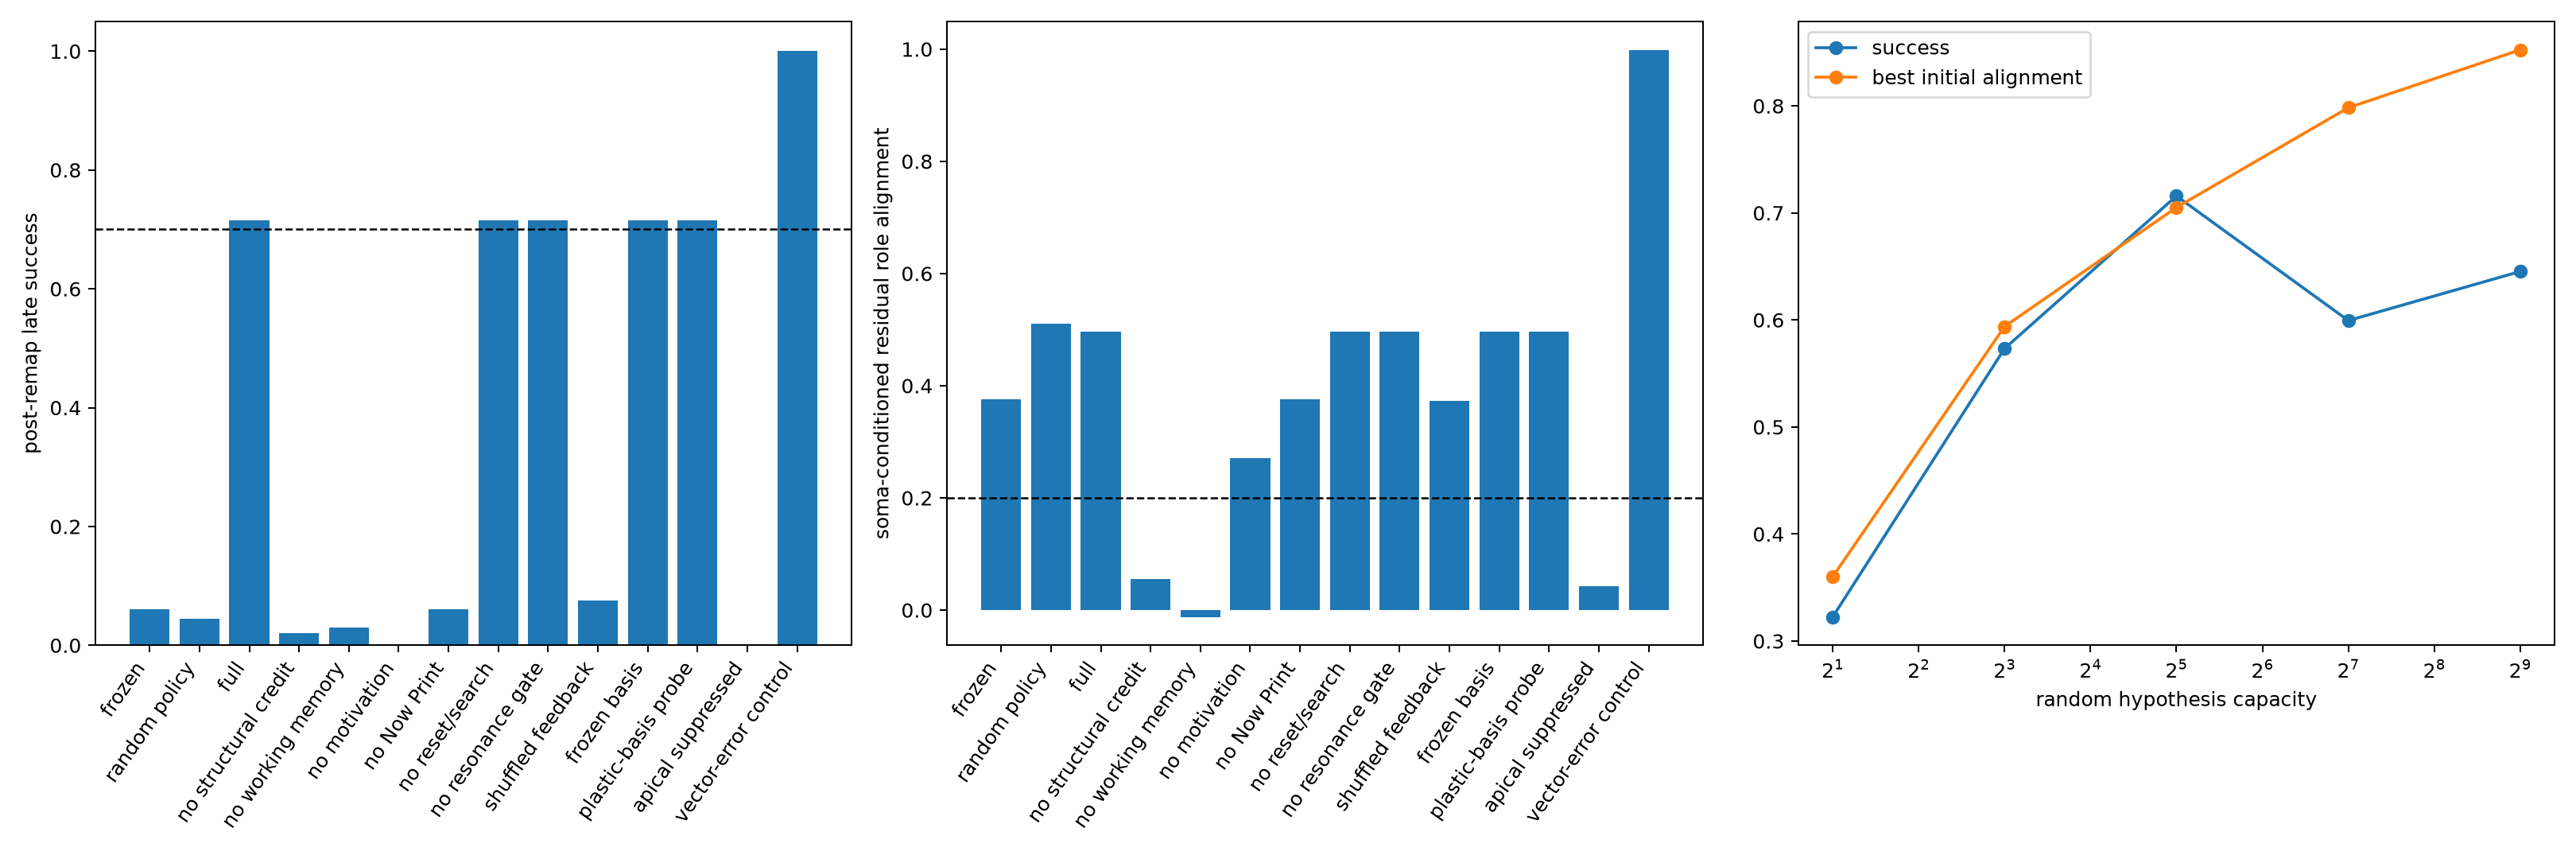
\includegraphics[width=\linewidth]{../results/exp001/frozen_v1/exp001_confirmatory.png}
\caption{Frozen random-repertoire comparison. The left panel shows post-remap success by condition, and the center panel shows soma-conditioned residual alignment. The right panel relates success and the best initial role alignment to hypothesis-bank capacity. The capacity relation is consistent with selection from a fixed repertoire rather than de novo cellular sign discovery.}
\label{fig:repertoire}
\end{figure}

\subsection{Learning a top-down expectation}
The learned-expectancy study (EXP002) asked whether repeated experience with selected patterns could produce a useful top-down signal. It added a Grossberg outstar-derived association,
\begin{equation}
T_h\leftarrow T_h+\eta(S_{\sim}-T_h),
\end{equation}
This equation moves the expectation $T_h$ toward the somatic pattern $S_{\sim}$ repeatedly active with the selected hypothesis. The expectation was learned and could be relearned after remapping. The behavioral scores and top-down alignments are reported in Table~\ref{tab:supporting}.

These behavioral results did not establish that the learned expectation carried a cellular teaching signal. Directly copying the selected pattern produced similar alignment, and a contextual bandit matched the behavioral performance. The main within-cell test also failed. Before and after remapping, the dendritic residual effects were $-0.326$ and $-0.016$. The corresponding effects in the neuron-indexed positive control were 0.660 and 0.545. Suppressing expectation learning removed the alignment of the learned pattern but had little effect on behavioral performance.

The model could store an expectation, but the expectation did not yet explain later cell-specific change. The next step was to test whether matched feedback could control local plasticity.

\subsection{Testing local plasticity and the complete model}
The local-mechanism study began with a comparison to the published theory (EXP003) and then tested a reduced SMART-inspired motif (EXP003a). It asked a narrow question. Could supplied matched feedback alter spike timing, permit a local weight update, and change a later feedforward response? The model did all three. The update and spike-probe results are reported in Table~\ref{tab:supporting}. No update occurred under competitor, top-down-ablated, or mismatch conditions. This result established the proposed local sequence when the appropriate feedback signal was supplied. It did not explain how the system learned that signal.

The complete model (EXP003b) combined this local mechanism with delayed structural credit and learned expectations. Across 12 held-out mappings, feedback advanced local spike timing and changed lower weights. Removing SMART input, the learned expectation, or local learning eliminated the effect. The timing result is reported in Table~\ref{tab:supporting}.

However, the model failed its main preregistered test. The early dendritic residual did not predict the later weight change or the later somatic change well enough to meet the predefined threshold. The neuron-wise positive control did complete this predictive chain. A post-hoc analysis then asked where the prediction was lost. The learned expectation $T$ and variables close to the plasticity rule predicted the sparse weight changes, but the soma-conditioned residual did not. Raw $T\rightarrow\Delta W$ correlation was 0.416 [0.290, 0.530]. Residual $D\rightarrow\Delta W$ correlation was $-0.004$ [$-0.141$, 0.128]. This analysis did not change the failed classification. Instead, it pointed to two separate questions. Where did the expectation's topology come from, and did the residual measure preserve the relevant information?

\subsection{Tracing the learned neuron pattern}
The topology study (EXP004) asked whether the complete model constructed a neuron-by-neuron pattern or instead inherited one from its fixed repertoire. The test varied the quality of the best pattern available before learning. Better initial coverage produced better behavior and better alignment between the learned expectation and the hidden roles (Figure~\ref{fig:topology}). At bank size $M=16$, the behavioral difference between high and low coverage was 0.197 [0.137, 0.255]. The corresponding scores and alignments are reported in Table~\ref{tab:supporting}.

A constructed sequential condition showed that the model could combine behavior across steps. Its performance reached 0.980 and exceeded the best repeated-single action by 0.313 [0.260, 0.374]. However, a contextual bandit reached 0.977. Behavioral composition alone therefore did not show that the model had constructed a new cellular topology.

The source of the learned pattern became clear through a comparison with experienced activity.
\begin{equation}
\mathrm{corr}(T,\text{selected initial soma})=0.999851,\qquad
\mathrm{corr}(T,\text{mean target})=0.999870.
\end{equation}
Exact replay reconstructed $T$ with RMSE 0.0, and $T$ did not surpass the best individual target that the model had experienced. Permuting outcomes changed which hypotheses and targets were visited, accounting for most of the change in topology. The outstar learned from selected states, but the neuron-by-neuron coordinates of those states came mainly from the fixed repertoire. Learning an arbitrary cellular topology would require a cell-varying quantity that was not already present in a candidate pattern.

\begin{figure}[tbp]
\centering
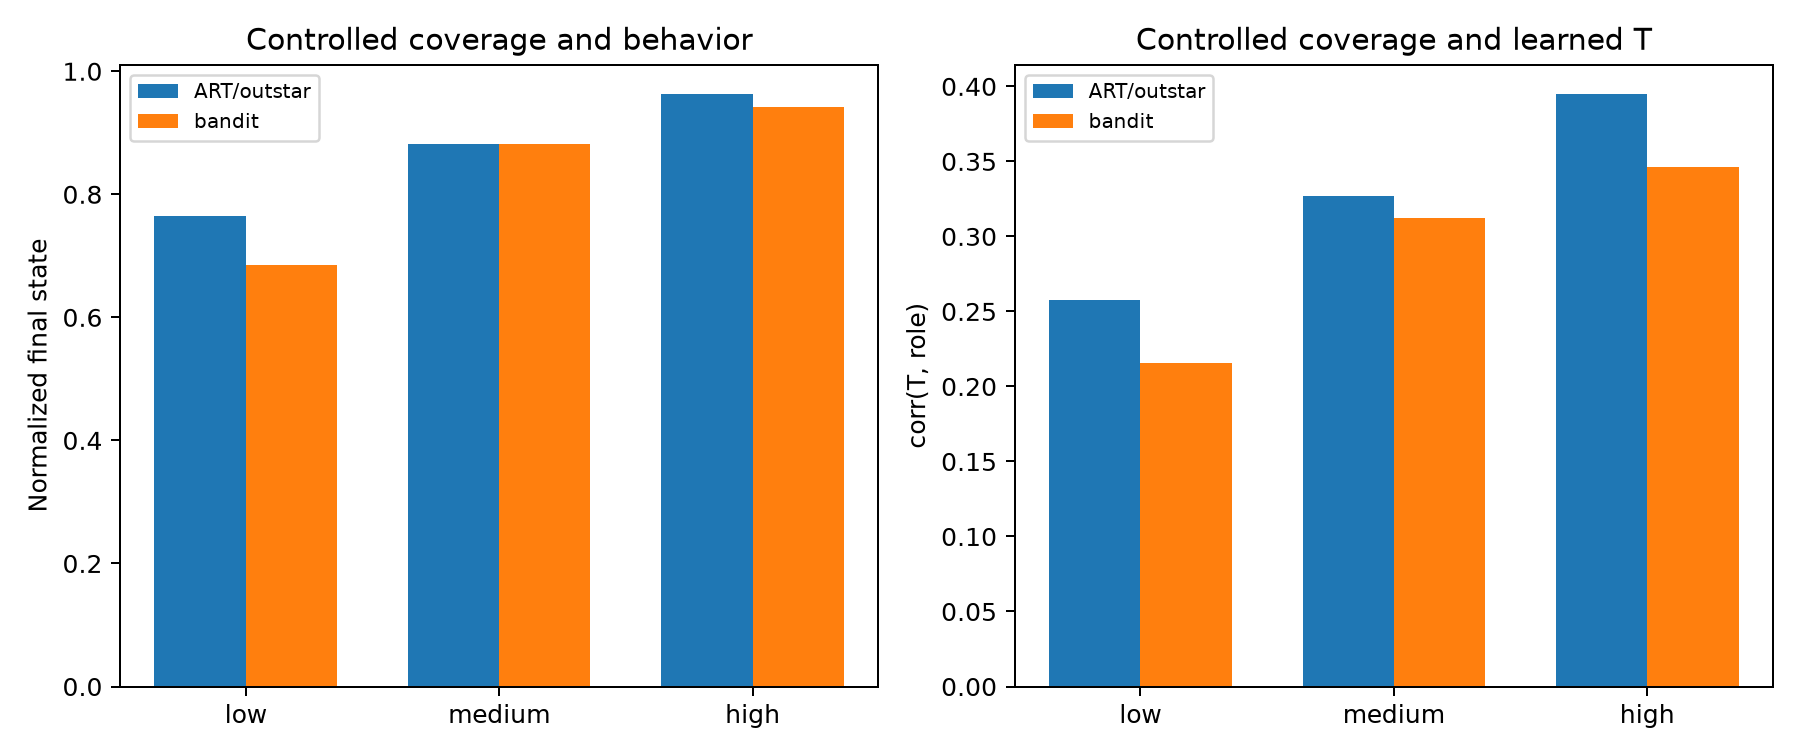
\includegraphics[width=\linewidth]{../results/exp004/frozen_v1/figures/controlled_coverage.png}
\caption{Frozen controlled-coverage result. Both final behavior (left) and alignment of the learned top-down expectation $T$ with hidden roles (right) increase with the quality of topology already available in the bank. The contextual-bandit comparison follows the same trend.}
\label{fig:topology}
\end{figure}

\subsection{Testing a local eligibility trace}
The next study (EXP005) first asked whether a published Grossberg equation supplied the missing cell-varying quantity. pART, ART/outstar learning, exploration, SMART, and vector motor systems each provided a related component. None of the inspected sources combined an independent local exploratory trace with a delayed scalar outcome to learn arbitrary intermingled signs. We therefore did not construct another model and label it as a Grossberg model.

Instead, a separate generic comparator tested whether that additional operation was computationally sufficient. After each exploratory change, each cell retained a private eligibility trace $e_i$. A later scalar outcome strengthened changes that had helped and reversed changes that had hurt. No hidden role information entered the update.

The comparator learned the hidden signs across all four tested population sizes and relearned them after an independent remap (Table~\ref{tab:eligibility}). At $N=32$, alignment reached 0.987 after acquisition and 0.964 after remapping. The learning curve rose quickly, fell when the hidden map changed, and rose again as the new map was learned (Figure~\ref{fig:eligibility}). Shuffling the outcome reduced post-remap alignment to 0.229. Removing plasticity, the temporal eligibility trace, or exploration left alignment near zero. The difference between the generic and shuffled conditions was 0.735 [0.655, 0.820].

Exact replay reproduced the updates to numerical precision. Final topology also exceeded the best single exploratory sample at every population size. The comparator therefore accumulated information across trials rather than selecting one fortunate perturbation. The scalar reward carried no more information than before. The new information came from the local trace, which allowed the same reward to produce different updates at different cells.

\begin{table}[tbp]
\centering\small
\begin{tabular}{L{0.23\linewidth}L{0.47\linewidth}L{0.20\linewidth}}
\toprule
Study & Supporting comparison & Result \\
\midrule
Routing & Accuracy with category and value learning frozen & 0.978 \\
Routing & Stored-category matches on ordinary corrected trials & 100\%, no resets \\
Learned expectation & Behavior before and after remapping & 0.528, 0.397 \\
Learned expectation & Top-down role alignment before and after remapping & 0.343, 0.287 \\
Local plasticity & Modeled update and learning-off spike probe & $0.600\rightarrow0.731$ and $0\rightarrow7/8$ \\
Complete model & Feedback-induced advance in local spike timing & 6.29 ms \\
Topology & Behavior at low, medium, and high initial coverage & 0.765, 0.882, 0.962 \\
Topology & Learned-$T$ alignment at the same coverage levels & 0.258, 0.327, 0.395 \\
\bottomrule
\end{tabular}
\caption{Supporting quantitative results from the theory-led studies.}
\label{tab:supporting}
\end{table}

\begin{table}[tbp]
\centering\small
\begin{tabular}{rrrr}
\toprule
$N$ & Acquisition alignment & Post-remap alignment & Changed-cell sign reversal \\
\midrule
8  & 0.997 & 0.968 & 1.000 \\
16 & 0.993 & 0.960 & 1.000 \\
32 & 0.987 & 0.964 & 1.000 \\
64 & 0.972 & 0.950 & 0.975 \\
\bottomrule
\end{tabular}
\caption{Generic local-eligibility results across population sizes. Each value summarizes 16 held-out maps after 1,280 acquisition episodes and 2,560 remap episodes.}
\label{tab:eligibility}
\end{table}

\begin{figure}[!t]
\centering
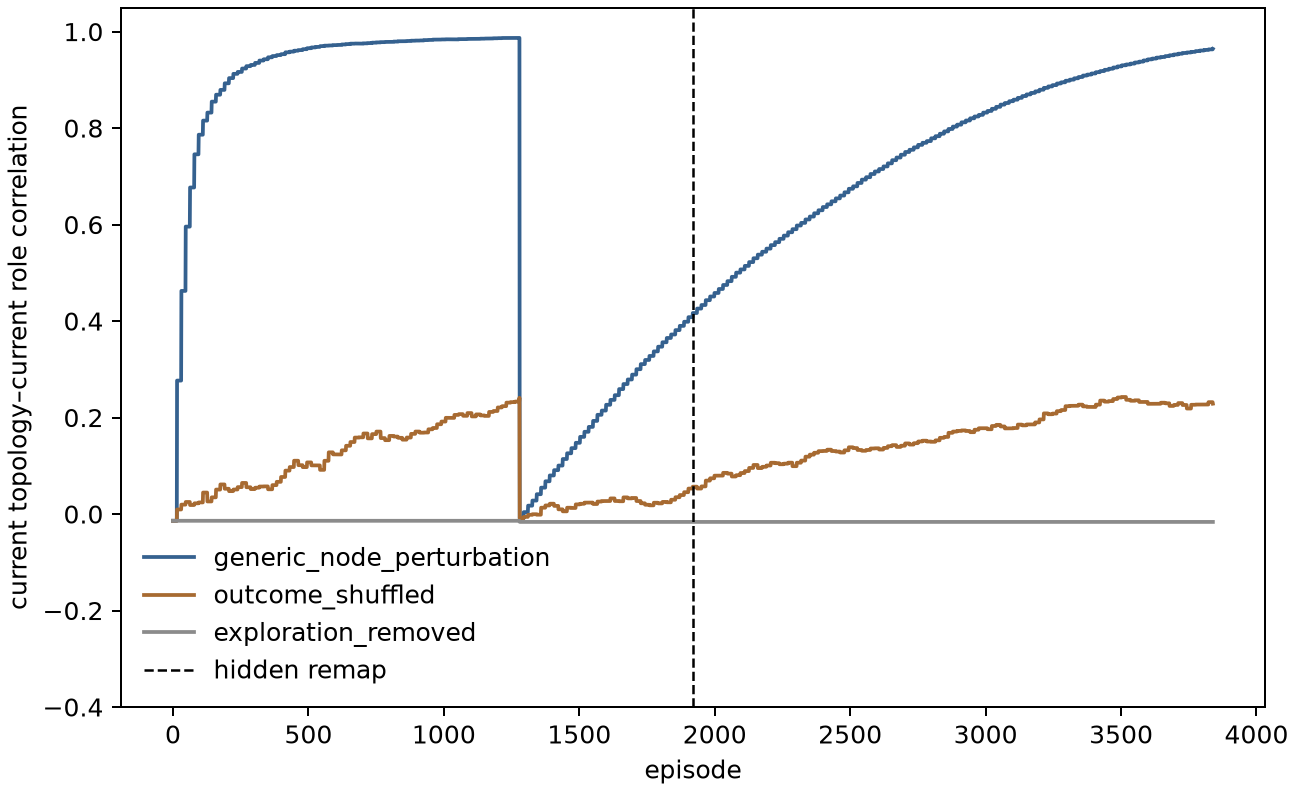
\includegraphics[width=0.82\linewidth]{../results/exp005/frozen_generic_v1/figures/n32_acquisition_trajectory.png}
\caption{Frozen generic local-eligibility diagnostic at $N=32$. The role alignment learned from scalar outcome and local perturbation eligibility rises during acquisition, drops when the hidden map changes, and is relearned. Shuffled outcome learns only weak alignment, while removing exploration eliminates learning.}
\label{fig:eligibility}
\end{figure}

\subsection{Comparing the mechanisms in one common benchmark}
The final study corresponds to registry record EXP006. It returned to the motivating question under one task, one observation model, and one frozen classification rule. The vector oracle, ART repertoire learner, local-eligibility learner, direct hybrid, and random control were tested on 32 previously untouched mappings with $N=10$.

Only the privileged vector oracle passed the complete bridge (Table~\ref{tab:exp006-classification}). This result establishes that the task and analysis could express every frozen endpoint when the correct cell-wise direction was supplied. It does not make the oracle biologically plausible.

The ART learner passed behavior and topology. Its late success was 0.675 during acquisition and 0.744 after remapping. Its topology correlations were 0.613 and 0.663. The latent role-by-direction scores were 0.513 and 0.613, and the measured residual scores were 0.030 and 0.039. The residual effect remained positive after matching somatic activity. Outcome decoding also passed. However, the early residual did not predict the later activity change during acquisition. The prospective score was $-0.203$ [$-0.396$, $-0.010$]. ART therefore failed the frozen Francioni-like signature. Its final topology was also below the best pattern already available in its fixed bank. This is evidence for learned selection, not for de novo cellular credit.

The eligibility learner reached acquisition success of 1.000 and remap success of 0.656. It constructed a strong acquisition topology with correlation 0.985. Remap correlation reached only 0.489, and changed-cell sign reversal reached 0.673. Both missed their frozen floors. Its latent and measured role-by-direction signals were near zero, and outcome decoding remained close to chance. Thus, the learner demonstrated substantial neuron-specific adaptation without reproducing the dendritic signature.

The hybrid passed behavior and topology. Its acquisition and remap success were 1.000 and 0.905. Its topology correlations were 0.878 and 0.763. The dendritic criteria nevertheless failed. The combined latent scores were $-0.119$ and $-0.088$. The measured residual scores were $-0.018$ and $-0.013$. Component archiving located the conflict. The ART component was positive at 0.555 and 0.591, whereas the eligibility component was negative at $-0.127$ and $-0.096$. Combining two useful behavioral operations did not automatically create the observed Francioni-like signal (Figure~\ref{fig:exp006}).

All five frozen control comparisons passed. Shuffling outcomes abolished ART success and strongly reduced eligibility learning. Removing exploration or the temporal trace abolished local-eligibility learning. Enabling eligibility in the hybrid improved acquisition success by 0.323 and acquisition topology by 0.278 over the hybrid without eligibility plasticity. Exact component reconstruction error was zero in every condition.

\begin{table}[tbp]
\centering\small
\begin{tabular}{L{0.30\linewidth}cccc}
\toprule
Model & Behavior & Topology & Dendritic signature & Full bridge \\
\midrule
Vector oracle & Pass & Pass & Pass & Pass \\
ART repertoire & Pass & Pass & Fail & Fail \\
Local eligibility & Pass & Fail & Fail & Fail \\
ART plus eligibility & Pass & Pass & Fail & Fail \\
Random no learning & Fail & Fail & Fail & Fail \\
\bottomrule
\end{tabular}
\caption{Frozen EXP006 classification for the primary $N=10$ benchmark. The dendritic column combines the preregistered latent vectorization, measured residual, outcome-decoding, and prospective-prediction criteria.}
\label{tab:exp006-classification}
\end{table}

\begin{figure}[tbp]
\centering
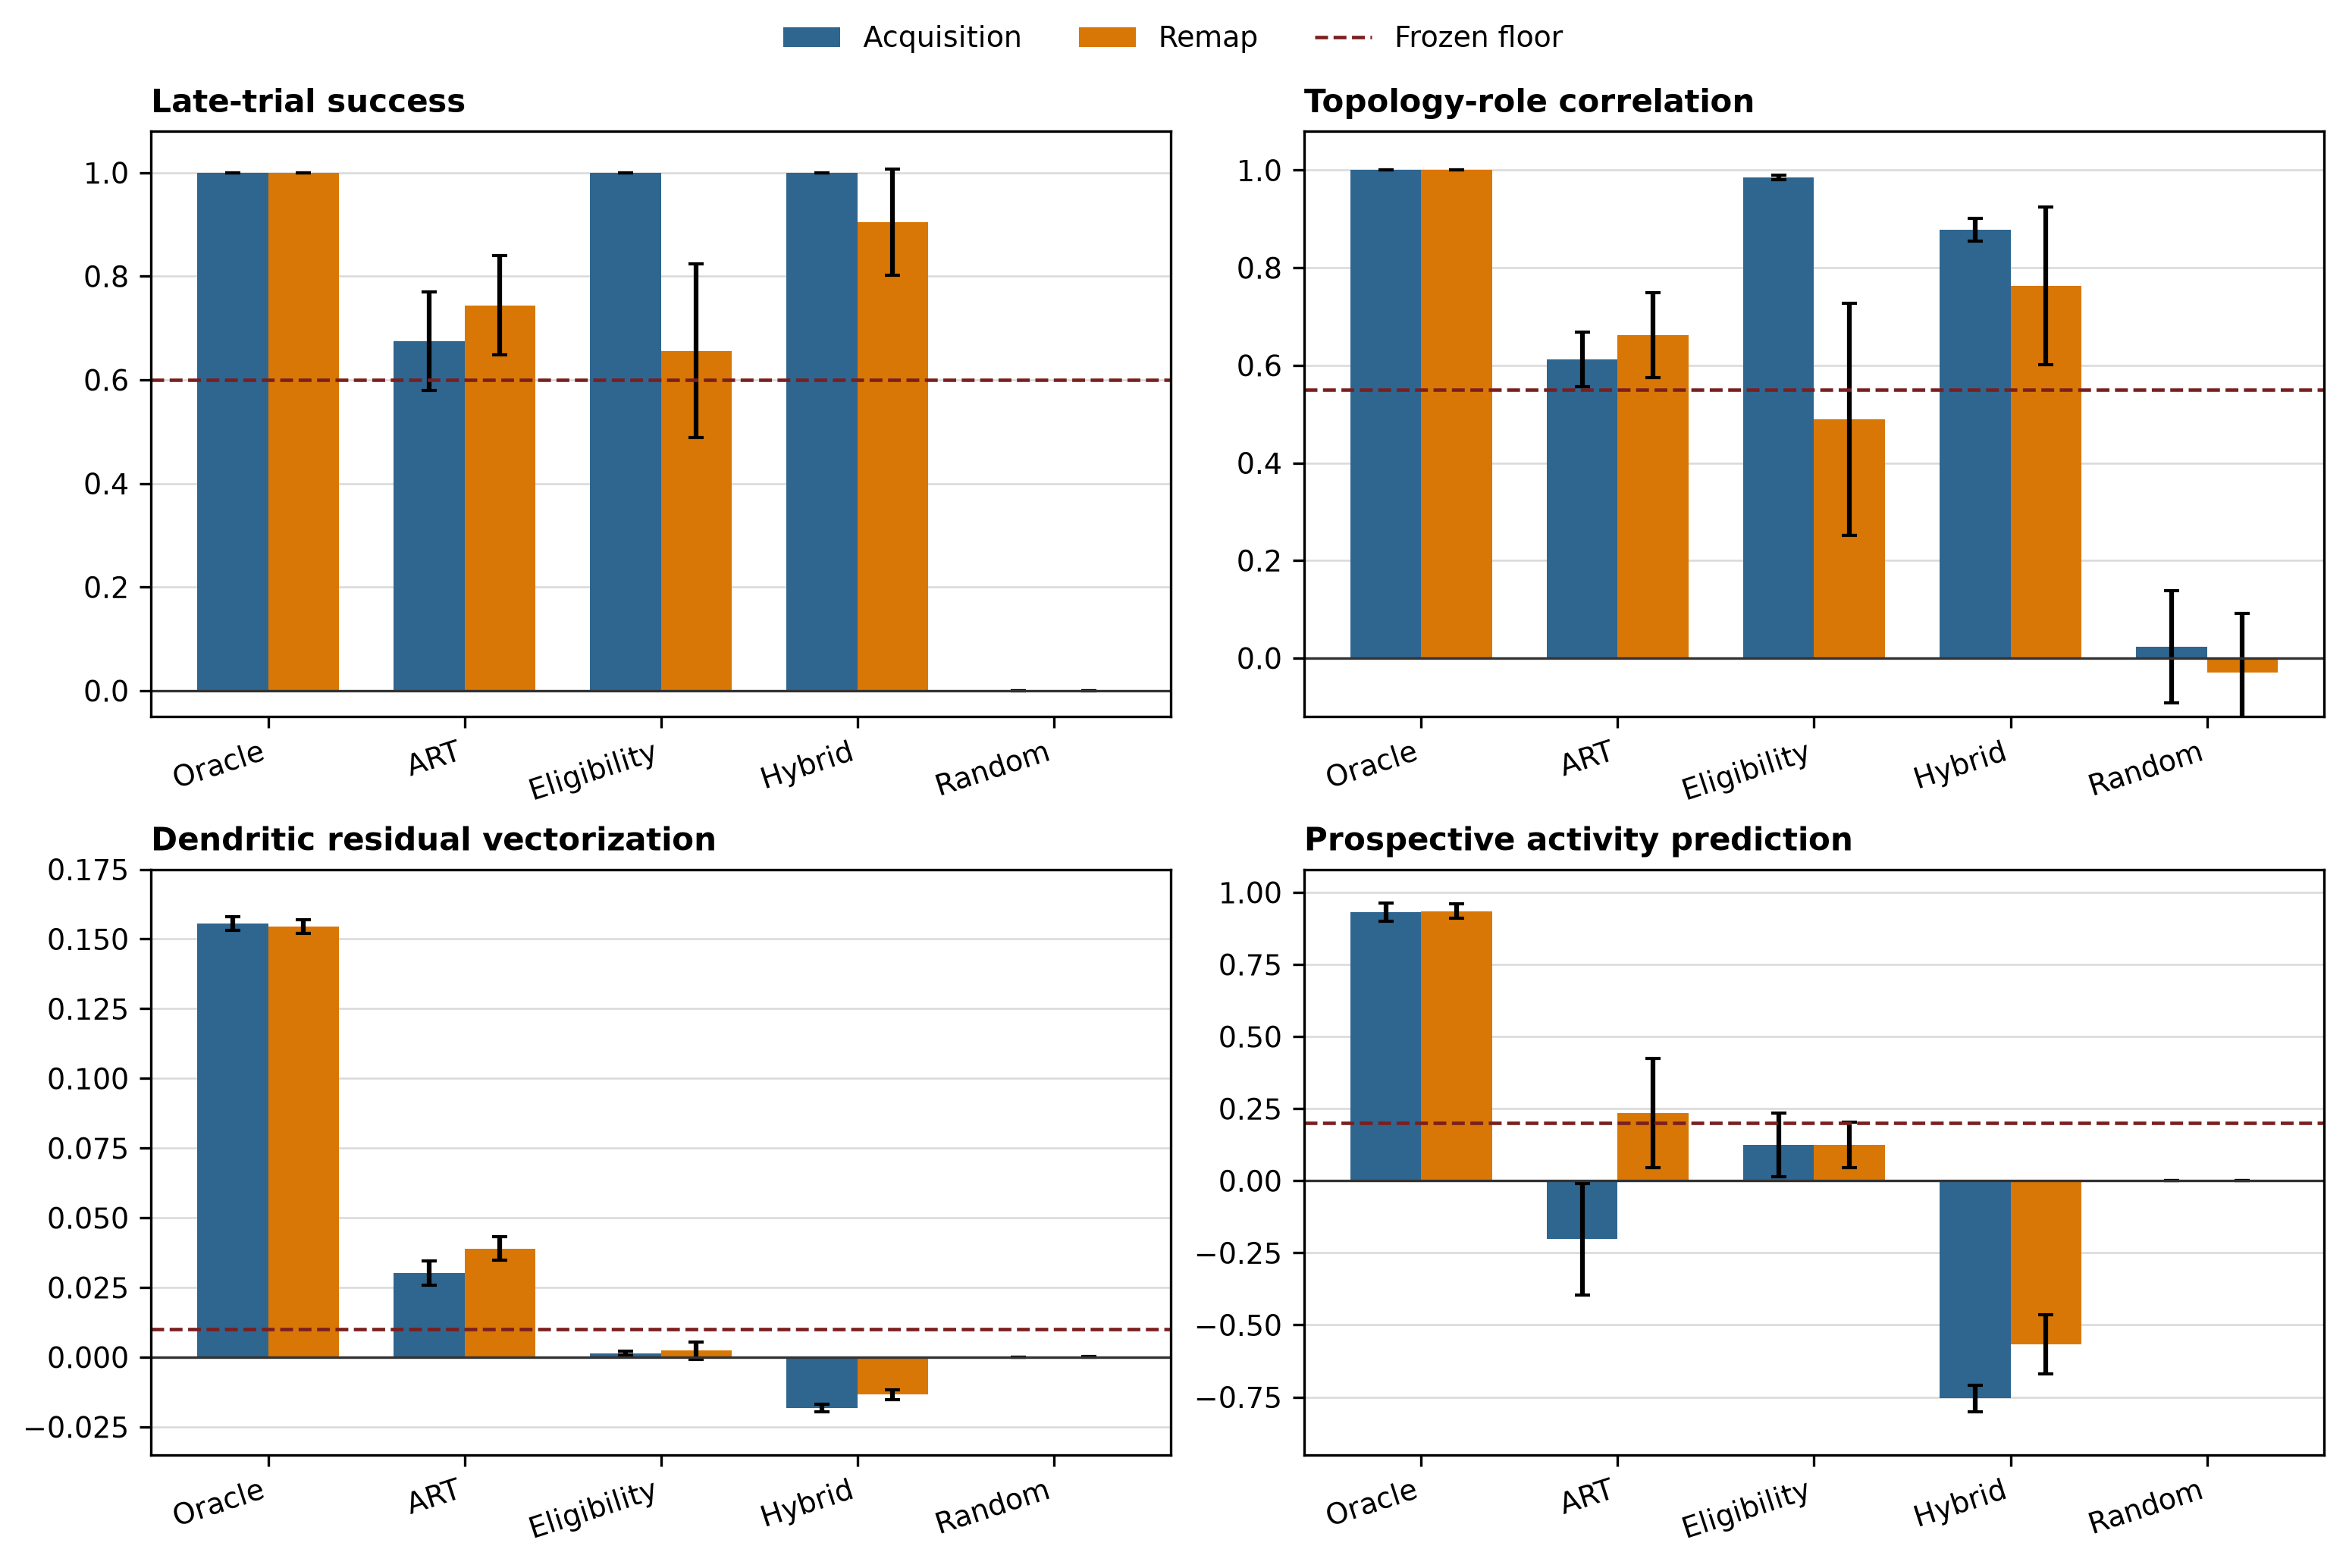
\includegraphics[width=\linewidth]{../results/exp006/frozen_v1_primary/figures/model_dissociation.png}
\caption{Frozen EXP006 primary result. ART, local eligibility, and the hybrid all improve behavior, but they differ in topology and dendritic endpoints. Dashed lines mark the prospectively frozen floors. Error bars show 95\% intervals across 32 held-out mappings.}
\label{fig:exp006}
\end{figure}

The predeclared $N=8$ check retained the main ordinary-model pattern. Every ordinary learner again failed the complete dendritic criterion. It was not a clean replication of the composite classification because even the vector oracle missed the pre-outcome decoding floor. The smaller task also made repertoire coverage unusually favorable. A bank of 64 patterns contains nearly all 70 possible balanced eight-cell patterns. The $N=8$ result is therefore a qualitative robustness check rather than a second primary test.

\FloatBarrier
\section{Discussion}
\subsection{What the study shows}
The experiments separate two kinds of learning that can produce similar behavior. Scalar reinforcement was enough to select and maintain useful population patterns. It also supported learned expectations and remapping. However, the neuron-by-neuron structure expressed by the ART-style models came mainly from patterns that were already available for selection. Selecting a successful representation is not the same as learning how each cell should change.

The common benchmark makes this distinction harder to dismiss as a difference between tasks. Under identical feedback and evaluation, ART passed behavior and selected role-aligned patterns from its bank. Local eligibility learned a new acquisition topology. The hybrid combined these abilities and learned fastest, but it failed the complete dendritic criterion. A model can therefore solve behavior and topology without reproducing the measured cellular signature.

\subsection{Are error-driven and ART-style accounts describing the same process?}
The original motivation was to ask whether they could be. The results give a qualified answer. At the level of behavior and population selection, they can look similar. Both an error-driven learner and a representation-selection system can improve performance and adapt after a contingency changes. At the cellular level, they are not interchangeable in the tested implementations. A role-specific error or target already contains cell-varying information. A pART-selected representation identifies which distributed state deserves credit, but it does not automatically create the missing coordinates of that state.

This does not make the two accounts incompatible. They may describe different levels of one learning system. An ART-like mechanism could stabilize context, select a causal representation, and preserve it until an outcome arrives. A separate cellular mechanism could then determine how eligible synapses or neurons change. That second mechanism might use an explicit vectorized instruction, a local perturbation trace, a dendritic target, or a combination of these signals. The experiments rule out equivalence for the specified pART-inspired bridge. They also show that one direct hybrid is insufficient. They do not rule out other hybrid architectures.

The failed longitudinal tests are important for the same reason. The earlier complete model produced learned expectations, altered spike timing, and changed local weights. Nevertheless, its soma-conditioned dendritic residual did not predict later change. In EXP006 the hybrid learned behavior and topology, yet its ART and eligibility components contributed opposite signs to the common dendritic proxy. These failures do not contradict the Francioni experiment, and they do not falsify ART or SMART. They show that assembling individually useful components is not enough. A model must explain how the correct cell-specific information is created, combined, and preserved in the measured dendritic variable.

\subsection{Relation to perturbation and three-factor learning}
The generic comparator showed how one scalar outcome can support different updates at different cells. Every cell received the same reward signal, but each combined it with a private memory of its own recent perturbation. Over repeated trials, these local associations formed the hidden neuron-by-neuron pattern. A centrally routed vector error was therefore not mathematically necessary in this abstract task.

This result agrees with established perturbation and three-factor learning. Dynamic node perturbation can estimate useful gradients from changes in a global objective \citep{fiete2006}. Eligibility traces can retain local pre- and postsynaptic information until a later modulatory event \citep{izhikevich2007,gerstner2018}. Reward-modulated Hebbian learning has also reproduced selective reorganization in an earlier BCI model by combining global reward with neuronal noise \citep{legenstein2010}. The local-eligibility study should be read as a controlled application of that known principle, not as the discovery of node perturbation.

Its contribution is diagnostic. The earlier abstract task exposed a repertoire limitation in the pART-inspired model. Adding a local perturbation trace supplied the kind of cell-varying information that was absent. Outcome shuffling, removal of exploration, and removal of eligibility eliminated the effect. EXP006 then showed why this sufficiency result should not be overextended. Local eligibility learned a strong acquisition topology, but it remapped incompletely and its within-trial update drive did not resemble the Francioni residual. The comparison locates a computational boundary. It does not yet provide a biological bridge across it.

\subsection{Measurement and attribution boundaries}
The complete models also revealed a measurement problem. Information can be present in a learned expectation, an eligibility drive, a current, or a spike-timing variable and still be absent from the measured calcium residual. EXP006 used one common observation layer and archived the latent signal separately from the measured residual. This distinguished an algorithmic failure from a measurement failure, but it did not make the synthetic layer biological. Future studies should state in advance which variable is expected to cause learning and how that variable should appear in dendritic recordings.

The comparison with published theory also sets an important boundary. A model may resemble pART or SMART without every component following from those theories. The cited work motivates representation selection, learned expectations, matching, and local plasticity. The exploratory eligibility rule adds a new hypothesis. It should be tested as a separate mechanism rather than attributed to Grossberg.

The present results also leave the biological interpretation open. Francioni's signal could reflect neuron-specific instruction, local error computation, matched top-down influence, eligibility for later reinforcement, or another dendritic operation. The current simulations compare the information required by these accounts. They do not identify the biological signal with any one of them.

\section{Limitations}
These tasks are abstract simulations. They do not reconstruct retrosplenial circuitry, animal behavior, calcium kinetics, or the complete equations of pART and SMART. Several biological links remain assumptions. These include connecting a pART-selected representation to a SMART-like projection, targeting the relevant BCI cells, mapping center/surround organization onto NDNF circuitry, and converting modeled activity into a calcium residual. The first routing model also begins with a favorable structure. The random-repertoire and outstar results depend on the particular pattern banks and ownership rules that were tested.

The common dendritic layer deliberately maps each model's internal cell-indexed quantity into the same synthetic observation. A positive result shows that the quantity can survive this chosen transformation. It does not show that real dendrites implement the quantity or that real calcium follows the same equation. A negative result can reflect the learning mechanism, the chosen internal variable, or their mapping into the observation layer. The positive oracle and separately archived latent signals make these possibilities visible but do not eliminate them.

The complete model used sparse, quantized local plasticity. Later analyses help explain why its main test failed, but they do not change the original classification. The local-eligibility comparator uses a population-size correction that contains no hidden role information. Even so, success in a finite, normalized task does not show that the rule would scale biologically. EXP006 tested one ART implementation, one eligibility rule, and one direct hybrid. Its negative full-bridge result does not apply to every ART model or every possible combination.

The secondary $N=8$ benchmark was sensitivity-limited because the vector oracle missed one decoding floor. Its repertoire also covered nearly all possible balanced patterns, which weakened its ability to distinguish selection from construction. The $N=10$ result is therefore primary. Finally, this manuscript synthesizes repository-derived computational records. It is not an independent reproduction or peer review of either the simulations or the motivating animal experiment.

\section{Biological predictions and discriminating tests}
The competing explanations make different experimental predictions.
\begin{enumerate}
\item \textbf{Interaction between eligibility and outcome.} A cell-specific deviation before the outcome should leave a local trace. The interaction between that trace and the later scalar outcome should predict the sign of plasticity. Disrupting the interval between the deviation and the outcome should impair learning without eliminating the scalar reward response.
\item \textbf{Remapping within the same cell.} If selected feedback determines the expressed pattern, a change in context or reward contingency should reorganize feedback before later somatic activity changes. The same cell should also be able to reverse its role across contexts.
\item \textbf{Dissociation between selection and cellular adaptation.} Restricting the available population repertoire should selectively impair an ART-like selection account. Reducing cell-specific variability while preserving the population state should selectively impair an eligibility account. A combined system should show both effects.
\item \textbf{Measurement of center and surround.} Excitatory feedback and NDNF-associated inhibitory surround should be measured and perturbed independently. This would test whether the predictive signal is a signed membrane effect rather than an excitatory calcium signal alone.
\item \textbf{Intervention at a specific projection and time.} A candidate feedback source should be perturbed before the outcome while sensory error and reward are preserved. This would show whether that projection carries cell-specific information. Broad suppression of activity would be harder to interpret.
\end{enumerate}
Together, these tests could distinguish among cell-specific instruction, selection of an available population pattern, and credit computed from a local exploratory trace.

\section{Conclusion}
This study began by asking whether an error-driven cellular account and an ART-style top-down population account might explain the same learning process. The experiments do not support equivalence. Scalar outcome was enough to select and maintain useful population patterns without a separate teaching value for every neuron. In the tested pART-inspired models, however, the neuron-by-neuron structure came mainly from representations that were already available. The earlier complete model also failed its preregistered test linking an early dendritic signal to later synaptic and somatic change.

A separate generic rule learned arbitrary cellular roles by combining scalar outcome with a local eligibility trace. The common benchmark then tested whether these operations jointly explained the motivating result. ART passed behavior and selected useful pre-existing patterns. Eligibility produced substantial cellular adaptation. Their direct hybrid passed behavior and topology, but its combined dendritic-like signal had the wrong sign. Only the privileged vector oracle passed every frozen criterion.

The central conclusion is therefore a computational dissociation. Selecting a causal representation and assigning credit to its individual cells are different operations. They may coexist in one biological system, but one does not automatically produce the other, and simply adding them is not yet an explanation of the Francioni signal. The most direct next step is to compare candidate mechanisms using the same biological measurements. A decisive experiment would test whether a cell's spontaneous or imposed deviation before the outcome leaves a local trace whose interaction with later reward predicts signed plasticity. In parallel, a more biophysical model should test how top-down, inhibitory, and local-eligibility signals combine and whether the result survives the calcium and soma-residual analysis used in the motivating experiment.

\section*{Data and code availability}
All computational results reported here derive from archived protocols, frozen analyses, held-out experiment records, and explicitly labeled post-hoc audits associated with this study. The EXP006 protocol, parameters, source hashes, endpoints, and numerical floors were committed before confirmatory execution. The public \href{https://github.com/OgnjenX/part-vector-credit}{project repository} provides the source code, experimental records, analysis outputs, and figure files used in this manuscript.

\bibliographystyle{plainnat}
{\small\setlength{\bibsep}{4pt}\bibliography{part_vector_credit_manuscript}}
\end{document}
